% \chapter{Analyse et Conception}
\chapter{Analyse des besoins}

\section{Introduction}
% Ce chapitre présente la partie conception qui sert à réaliser des différents types de
% diagramme qui modélise les différentes parties du projet afin de mieux comprendre l'application.


Dans ce chapitre , nous allons montrer les fonctionnalités de chaque acteur
avant de pouvoir passer à la conception de notre projet.
 \section{ Les besoins fonctionnels}
  \subsection{ Présentation des acteurs}
Premièrement, les acteurs sont des entités externes par rapport à un système modélisé et qui intéragissent avec ce système. Identifier les acteurs intervenant peut en fait représenter une véritable problématique. Pour nous aider à mieux les identifier, voici
quelques questions qui nous permettront plus facilement d'identifier les acteurs de notre système :
\vspace{0.2cm}
% \begin{enumerate}
% \item Third level, enumerate, first item
% \item Third level, enumerate, second item
% \end{enumerate}
\begin{enumerate}
\item Quels sont les utilisateurs qui ont besoin d'un système pour réaliser le
travail ?

\item  Quels sont les utilisateurs qui vont effectuer les actions principales du
système ?

\item Quels sont les utilisateurs qui vont exécuter les fonctions principales
du système (maintenance et administration) ?

\item Est-ce que le système interagit avec le matériel ou d'autres logiciels ?
\vspace{0.2cm}
\end{enumerate}
En se basant uniquement sur ces quatre dernières questions, nous pouvons
facilement identifier nos acteurs.
Pour notre système ,bien évidemment notre application web, nous avons
quatre acteurs :\\
\begin{itemize}
\item[$\bullet$] Le citoyen\\
\item[$\bullet$] L'empolyé\\
\item[$\bullet$] L'administrateur
\end{itemize}

\newpage
 \subsection{ Identification des fonctionnalités par acteur}
 Nous présenterons dans ce qui suit la fonction de chacun de nos utilisateurs :\\\\
\large{\textbf{      Fonctionnalité du citoyen : }}
 \newpage
 \section{ Les besoins non fonctionnels}
\begin{itemize}


\item[$\bullet$] \textbf{L'utilisation :}  L'application doit être facile à utiliser, être adaptée aux différents citoyens,  dont le but général est de les satisfaire.\\


\item[$\bullet$]\textbf{L’extensibilité :} l’application devra être extensible, c’est-à-dire qu’il pourra y avoir une possibilité d’ajouter ou de modifier des nouvelles fonctionnalités. \\

\item[$\bullet$] \textbf{La performance : }: Est l'une des premières exigences d'une application
web, et surtout les applications destinées au grand public. Ce dernier juge souvent
la performance par le temps de réponse de l'application, donc notre application doit
répondre rapidement aux actions des utilisateurs, et s'il y a un traitement qui peut
prendre de temps, il vaut mieux l'exécuter en arrière-plan.
\\

\item[$\bullet$] \textbf{L’interface :} Avoir une interface de bon niveau surtout que l’utilisation des Smartphones et des tablettes imposées que l’interface soit adaptative. \\




% \item[$\bullet$] \textbf{La convivialité :} L’application doit être simple et facile à manipuler par les utilisateurs.

\end{itemize}
% % Ce diagramme est classé comme un modèle statique du système, il sert à réaliser une
% % modélisation des relations entre les classes du système orienté objet.

% % \begin{figure}[!h]
% %   \centering
% %   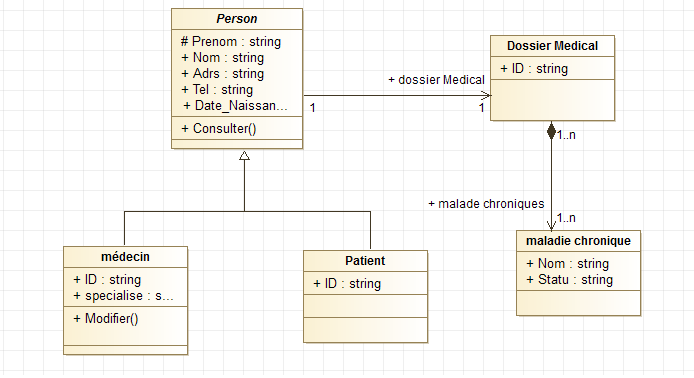
\includegraphics[width=15cm,height=15cm,keepaspectratio]{figure/seq/fig4.png}
% %   \caption{Diagramme de classes}
% % \end{figure}

% % La figure  présente le diagramme de classes de notre projet :

% % \begin{description}

% %   \item[Person : ] c’est la classe qui contient les informations generales sur les utilisateurs .
% %   \item[Patient : ]c’est une classe qui hérite de la classe  Person  et qui dispose des attributs et des opérations supplémentaires concernant le patient.
% %   \item[Medécin : ] c’est une classe qui hérite de la classe  Person  et qui dispose des attributs et des opérations supplémentaires concernant le médecin.
% %   \item[Dossier Medical : ] c’est la classe qui contient les informations médicales pour chaque patient  .
% %   \item[Maladie Chronique : ] c’est la classe qui contient la statut et les information de chaqun des maladies chroniques qui est dans le dossier medical  .

% % \end{description}

% \section{Diagramme de cas d'utilisation }
% Ce diagramme  capture le comportement d'un système,
% d'un sous-système, d'une classe ou d'un composant, il représente une interaction entre un
% utilisateur (humain ou machine) et un système, les utilisateurs sont appelés acteurs ils
% interagissent avec les cas d'utilisation.\\
% \begin{figure}[!h]
%   \centering
% 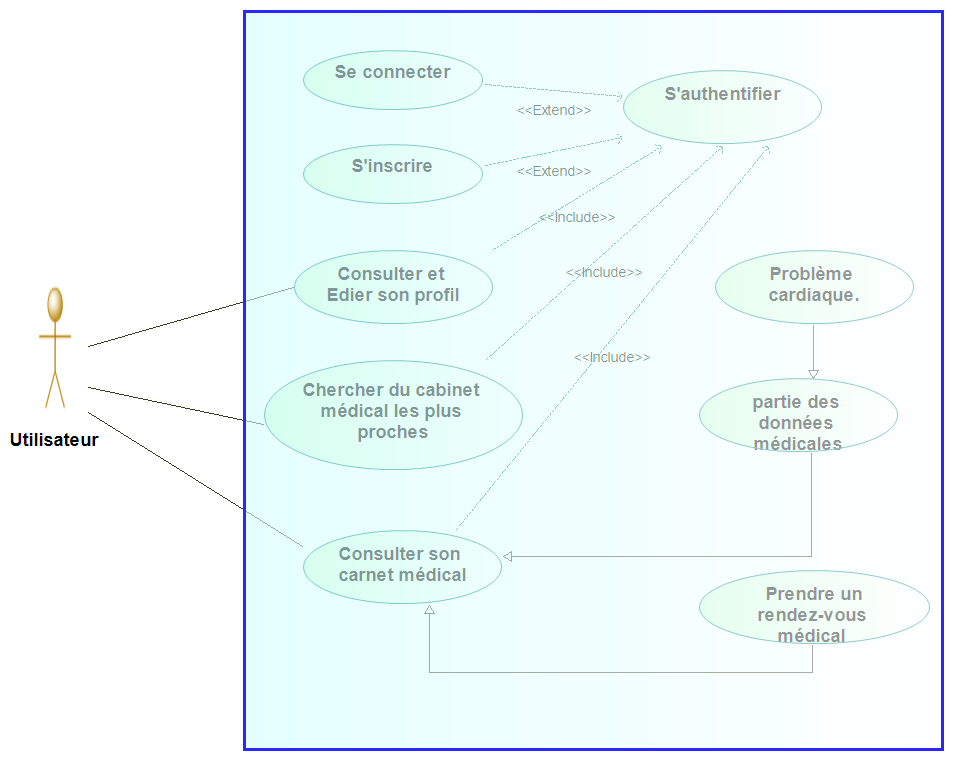
\includegraphics[width=15cm,height=15cm,keepaspectratio]{figure/fg9.png}
%   \caption{ Diagramme de cas d'utilisation}
% \end{figure}

% Le  diagramme  de cas  d'utilisation  ci-dessus  nous  montre  l'interaction  entre  l'utilisateur  et l'application , l'utilisateur doit s'authentifier pour  accéder à une page d'accueil .
% \newpage
% \section{Les diagrammes de séquences}
% Les diagrammes de séquence peuvent servir à illustrer les cas d’utilisations décrits dans la
% partie précédente . Ils permettent de représenter la succession chronologique des opérations
% réalisées par un acteur et qui font passer d’un objet à un autre pour représenter un scénario.
% Dans cette partie, nous allons décrire les scénarios les plus importants ainsi que leurs
% représentations par les diagrammes de séquence

% \subsection{Cas d’utilisation « Connection »  }
% \begin{figure}[!h]
%   \centering
% 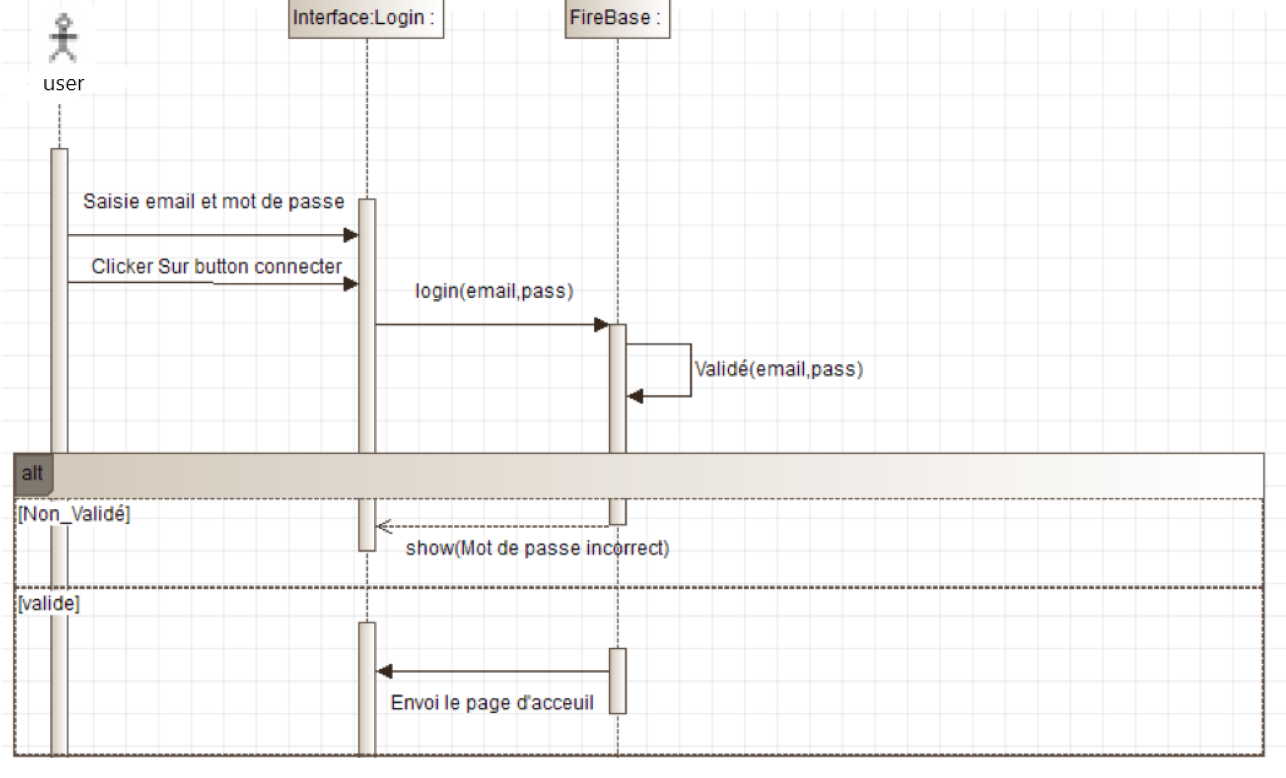
\includegraphics[width=15cm,height=20cm,keepaspectratio]{figure/seq/fig1.png}
%   \caption{Diagramme de séquence du cas d'utilisation "s'authentifier"}
% \end{figure}

% La figure  représente les différentes séquences qui se produisent lorsqu’un utilisateur
% appuie sur le bouton de connexion (Sing in) de l’interface d’authentification, le système  va
% tout d’abord tester s’il y a un champ vide ou invalide, après il va demander au serveur de Firebase de
% vérifier les informations d’authentification .
% \newpage
% \subsection{Cas d’utilisation « Inscription »  }
% \begin{figure}[!h]
%   \centering
% 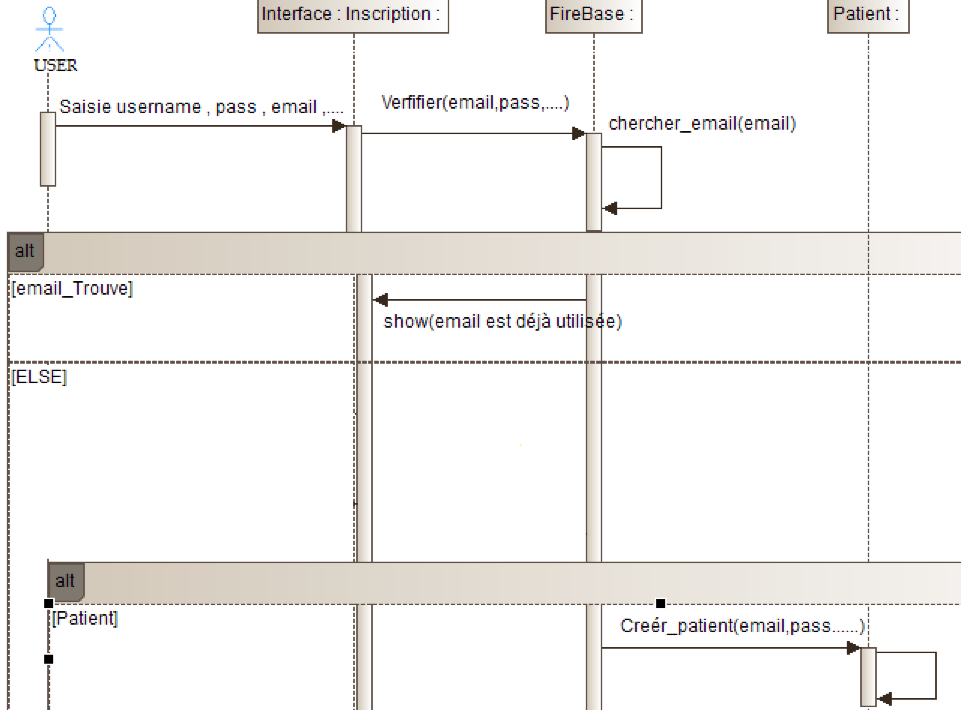
\includegraphics[width=15cm,height=20cm,keepaspectratio]{figure/seq/fig3.png}
%   \caption{Diagramme de séquence du cas d'utilisation "Inscription"}
% \end{figure}

% La figure  représente les différentes séquences qui se produisent lorsqu’un utilisateur
% appuie sur le bouton d'inscrir (Sing up) , le système  va
% tout d’abord tester s’il y a un champ vide ou invalide et si gmail a été déjà utilisé  après il va demander au serveur de Firebase de
% vérifier les informations d’inscrir puis creer un compte dans la base de donnée .
% \newpage
% \subsection{Cas d’utilisation « Password reset  »  }
% \begin{figure}[!h]
%   \centering
% 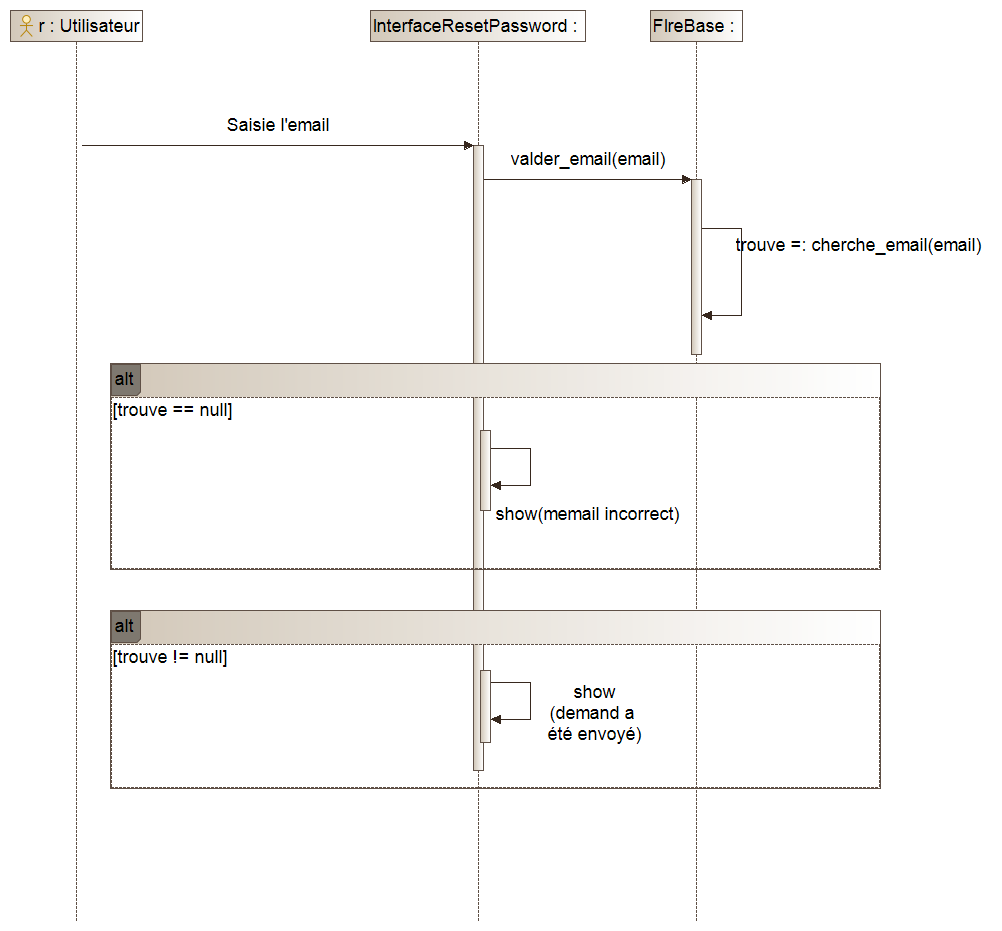
\includegraphics[width=15cm,height=20cm,keepaspectratio]{figure/seq/fig2.png} \\
%   \caption{Diagramme de séquence du cas d'utilisation "password reset "}
% \end{figure}

% La figure  représente les différentes étapes qui se produisent lorsqu’un utilisateur a oublué  son email, donc il faut à l'utilisateur  a envoyé son gmail pour reçois leur mot de passe à leur gmail.


% \section*{Conclusion }
% Ce chapitre a présenté la conception de notre application mobile. Nous
% avons détaillé la conception de notre application à travers  diagrammes de
% classe , diagrammes de cas d'utilisation ,  ainsi que Les diagrammes de séquences associées afin que la phase
% réalisation et la mise en place de l’application mobile soit plus souple et
% plus aisée. Cette conception a été faite en UML. \\
% Dans le chapitre suivant, nous  avons donné un aperçu sur l'ensemble des outils utilisés realiser cet application.
% % ,
% % framework et langages utilisés pour 